% Copyright 2022 Thomas Ascher
% SPDX-License-Identifier: CC-BY-SA-4.0

\documentclass[a4paper,parskip=half]{scrartcl}

\usepackage[T1]{fontenc}
\usepackage{mathpazo}
\usepackage{amsmath}
\usepackage[naustrian]{babel}
\usepackage{csquotes}
\usepackage{booktabs}
\usepackage{graphicx}
\usepackage{chemformula}
\usepackage{icomma}
\usepackage{gensymb}
\usepackage{float}
\usepackage[section]{placeins}
\usepackage[style=apa,backend=biber]{biblatex}

\usepackage[hidelinks,pdfencoding=auto,
  pdfauthor={Thomas Ascher},
  pdfusetitle,
  pdfkeywords={Bier,Farbe,Lovibond,SRM,EBC,Morey,Krüger}]{hyperref}
\usepackage{microtype}

\setkomafont{disposition}{\normalfont\bfseries}

\addto\extrasnaustrian{
\def\figureautorefname{Abb.}
\def\tableautorefname{Tab.}
\def\equationautorefname{Gl.}
}

\addto\captionsnaustrian{
\renewcommand{\figurename}{Abb.}
\renewcommand{\tablename}{Tab.}
}

\NewBibliographyString{gethesis}
\DefineBibliographyStrings{naustrian}{
  mathesis = {Masterarbeit},
  gethesis = {Diplomarbeit},
}

\newcommand{\MCUL}{\mathit{MCU}}
\newcommand{\MCUEBC}{\mathit{MCU}_{EBC}}
\newcommand{\EBC}{\mathit{EBC}}
\newcommand{\SRM}{\mathit{SRM}}
\newcommand{\ulovi}{\:[\textrm{°L}]}
\newcommand{\usrm}{\:[\textrm{SRM}]}
\newcommand{\uebc}{\:[\textrm{EBC}]}
\newcommand{\uebch}{\:[\textrm{EBC/h}]}
\newcommand{\uli}{\:[\text{l}]}
\newcommand{\ugal}{\:[\textrm{US gal}]}
\newcommand{\ukg}{\:[\textrm{kg}]}
\newcommand{\ulb}{\:[\textrm{lb}]}
\newcommand{\uplato}{\:[\textrm{°P}]}
\newcommand{\fstw}{f_{Stw}}
\newcommand{\khell}{k_{Hell}}
\newcommand{\kkd}{k_{Kd}}
\newcommand{\kstw}{k_{Stw}}
\newcommand{\uhour}{\:[\textrm{h}]}

\title{Es wird bunt: Bierfarbe aus der Schüttung berechnen}
\author{Thomas Ascher <thomas.ascher@gmx.at>}
\date{\today, \href{http://creativecommons.org/licenses/by-sa/4.0/}{CC BY-SA 4.0}}

\addbibresource{bierfarbe.bib}

\begin{document}
\maketitle

\section*{Einleitung}

Bernsteinfarben, Schwarz, Rot oder Braun: Abseits der blonden Lager existiert das Produkt Bier innerhalb eines weitreichenden Farbspektrums. Neben einem nicht weltweit normierten Vokabular, wie es zum Beispiel \autoref{table:bacolor} zeigt, werden auch verschiedene Skalen verwendet, um diese Farben zu beschreiben. Großteils verantwortlich für dieses Farbenspiel ist die in einem Rezept eingesetzte Malzmischung, die Schüttung. Wie aus dieser die zu erwartende Bierfarbe näherungsweise berechnet werden kann, wird in den folgenden Abschnitten dieses Artikels demonstriert.

\begin{table}[H]
\centering
\begin{tabular}{lr}
\toprule
\multicolumn{1}{c}{\textbf{Farbbeschreibung}} & \multicolumn{1}{c}{\textbf{EBC}} \\
\midrule
Hellgelb & 1 \\
Strohgelb & 5 \\
Goldgelb & 10 \\
Bernstein & 15–20 \\
Kupfer & 25–30 \\
Hellbraun & 35–40 \\
Braun & 45 \\
Dunkelbraun & 50–55 \\
Schwarz & 60 \\
\bottomrule
\end{tabular}
\caption{EBC Wert für Farbeindrücke \parencite[34]{Bruecklmeier2018}}
\label{table:bacolor}
\end{table}

\begin{figure}[h]
\centering

\includegraphics[width=14cm]{colorscale.pdf}
\caption{Farbsimulation für die Werte der \autoref{table:bacolor} (Ascher, 2022)}
\label{fig:bacolorscale}
\end{figure}




\section*{Messung von Bier- und Malzfarbe}

Zur Bestimmung der Bierfarbe existieren mehrere Messskalen und Messverfahren. Die Älteste davon noch gebräuchliche, ist die Lovibond Skala. Diese wurde vom Brauer Josep W. Lovibond 1885 zusammen mit einem Messgerät, dem Tintometer, entwickelt. Damit wird per visuellem Eindruck von einer Person eine aufbereitete Bierprobe mit verschieden gefärbten Glasscheiben verglichen, um einen Messwert zwischen 2 bis 70~°L (hell bis dunkel) zu ermitteln. Unterschiede in der menschlichen Wahrnehmung und verschiedene Umwelteinflüsse verfälschen das Messergebnis. \parencite{KrausWeyermann2021a}

Im Jahr 1951 hat die \href{https://www.asbcnet.org}{American Society of Brewing Chemists (ASBC)} eine neue Analysemethode (Standard Reference Method) auf Basis des Spektrophotometers zusammen mit der SRM Skala, die an die Lovibond Skala gekoppelt ist, ratifiziert. Eine bedingte Umbrechnung zwischen °L und SRM ist durch \autoref{eq:ltosrm} und \autoref{eq:srmtol} möglich. Seit 1996 verwendet die \href{https://europeanbreweryconvention.eu}{European Brewery Convention (EBC)} die EBC Skala, die sich ebenfalls auf die Messwerte eines Spektrophotometers bezieht. Bis auf die Skala wurde die grundlegende Messmethode von beiden Normungsgremien mittlerweile harmonisiert. Bei dieser misst ein Spektrophotometer die Lichtabsorption einer entgasten Bierprobe oder eine aus einem Malz im Kongressmaischeverfahren hergestellten Würzeprobe bei einer Wellenlänge von 430~nm durch eine 1~cm breite Quarzglasküvette. Der 12,7-fache Logarithmus der gemessenen Absorption entspricht dabei einem Wert auf der SRM Skala und der 25-fache Logarithmus der Absorption einem Wert auf der EBC Skala. Daraus leitet sich der Zusammenhang von \autoref{eq:ebctosrm} ab. Das menschliche Auge kann Farbunterschiede ab 80~EBC nicht mehr wahrnehmen. Auch Messgeräte generieren darüber keine zuverlässigen Messwerte mehr. Dunkle Bierproben sind daher vor der Messung zu verdünnen. \parencite{KrausWeyermann2021a}

\begin{equation}
\textrm{°L} = 0,808 \cdot \SRM - 0,0083
\label{eq:ltosrm}
\end{equation}

\begin{equation}
\SRM = \textrm{°L} + 0,04662 \cdot \textrm{°L}^2
\label{eq:srmtol}
\end{equation}

\begin{equation}
\EBC = \SRM \cdot 1,97
\label{eq:ebctosrm}
\end{equation}

% TODO devices
\parencite{Fengxia2004}
\parencite{Caro2019}

„\href{https://bieranalyse.de}{Bieranalyse Fuchs}“

\section*{Modelle zur Schätzung der Bierfarbe}

Seit etwa der Mitte der Neunzigerjahre sind im Heimbraubereich mehrere Berechnungsmodelle entstanden, die versuchen aus den proportionalen Farbbeiträgen der Malze in eine Schüttung die zu erwartende Bierfarbe vorhersagen. Diese Beiträge bezeichnet \textcite[61]{Daniels1996} als „Malt Color Units (MCU)“, \textcite[34]{Mosher1994} als „Homebrew Color Units (HCU)“  und \textcite[10]{Holle2010} als „Würze SRM“, denn die MCU beschreibt bestenfalls einen Eindruck der Würzefarbe. Bei dieser Art der Berechnung wird nicht berücksichtigt, dass dunklere Malze überproportional zufärben \parencite{KrausWeyermann2021c}.

Aufgrund verschiedener Einflüsse während des Brau- und Gärprozesses benötigt es weitere Korrekuren um aus der MCU eine Schätzung der Bierfarbe zu erhalten. Folgende Faktoren führen unter anderem abseits der verwendeten Malzen zu einer dunkleren Bierfarbe: eine höhere Restalkalität des Brauwassers, eine feinere Schrotung, eine längere Maischedauer (Maillard-Rekation), der Einsatz intensiverer Maischeverfahren wie der Dekoktion, eine längere Kochdauer (Karamellisierung), eine höhere Stammwürze (Stw.) und eine stärkere Oxidation \parencites{KrausWeyermann2021c}[78]{Hanghofer2019}. Darüber hinaus haben auch die Trubbildung bei der Würzekühlung, der pH-Sturz während der Gärung und  Gärnebenprodukte der Hefen Einfluss auf die Bierfarbe. Die erste weit verbreitete Korrelation, die nur einen Bruchteil der genannten Faktoren berücksichtigt, stammt vom Heimbrauer Randy Mosher, wobei sich mittlerweile das Modell von Daniel Morey weitgehend als Standard im Heimbrauumfeld etabliert hat \parencite{KrausWeyermann2021b}. Eine genaue Vorhersage müsste alle Faktoren einbeziehen. Deshalb formulierte \textcite{Colby2000} die Notwendigkeit der Einführung einer „New Homebrew Color Unit (NHCU)“, die einen additiven und einen multiplikativen Korrekturfaktor beinhaltet.

Die Würzefarben von Braumalzen, die für die folgenden Berechnungen benötigt werden, sind üblicherweise auf den Webseite der jeweiligen Mälzereibetrieben einsehbar. Alternativ kann eine große Anzahl von Malzanalysedaten über die \href{https://obrama.mueggelland.de}{Obrama DB} von Jörg Krüger abgerufen werden. Notwendige Konvertierungen von SI-Einheiten zu United States Customary Units erfolgen \autoref{eq:kgtolb} und \autoref{eq:ltogal}.

\begin{equation}
\text{lb} = \frac{\text{kg}}{0,45359237}
\label{eq:kgtolb}
\end{equation}

\begin{equation}
\text{US gal} = \frac{\text{l}}{3,785411784}
\label{eq:ltogal}
\end{equation}

\subsection*{Burch (1993)}

In der erweiterten zweiten Ausgabe des Buchs „\citetitle{Burch2010}“ stellt \textcite[102]{Burch2010} das Berechnungsverfahren in \autoref{eq:mcuburch} vor. Er geht dabei von einer gesamten Maischedauer von 90~min aus. Nachdem das Buch von Burch von 1986 bis 2010 mehrere Überarbeitungen erfahren hat (auch innerhalb der selben Ausgabe), ist das Jahr der Veröffentlichung unklar.

\begin{equation}
\SRM = \frac{\sum \text{Malzgewicht}_i \ulb \cdot \text{Malzwürzefarbe}_i \usrm}{\text{Volumen kalte Anstellwürze} \ugal} 
\label{eq:mcuburch}
\end{equation}

\subsection*{Mosher (1994)}

Nicht als Gleichung sondern als Nomogramm ist das Modell von \textcite[34]{Mosher1994} ausgeführt. Die Datengrundlage dafür waren verfügbate Rezepte und Messwerte von kommerziellen Bieren \parencite{Morey2004}. Zur Berechnung nach Mosher ist die MCU nach \autoref{eq:mcubasis} zu bestimmen. Danach wird per Nomogramm der resultierende SRM Wert korreliert. Die \autoref{eq:mcumosher}, die anstatt des Nomogramms verwendet werden kann, wird von Morey Mosher zugeschrieben. In Moshers Buch „\citetitle{Mosher1994}“ ist diese aber nicht enthalten. 

\begin{equation}
\MCUL = \frac{\sum \text{Malzgewicht}_i \ulb \cdot \text{Malzwürzefarbe}_i \ulovi}{\text{Volumen kalte Anstellwürze} \ugal} 
\label{eq:mcubasis}
\end{equation}

\begin{equation}
\SRM = 0,3 \cdot \MCUL + 4,7
\label{eq:mcumosher}
\end{equation}

Später hat \textcite[258]{Mosher2015} in „\citetitle{Mosher2015}“ eine metrische Variante der \autoref{eq:mcubasis} mit dazugehörigem Nomogramm veröffentlicht. Diese unterscheidet sich von den Berechnungen der folgenden metrischen Modelle und dürfte im Heimbrauumfeld aber keine wesentliche Bedeutung erlangt haben.

\subsection*{Daniels (1995)}

In seinem Buch „\citetitle{Daniels1996}“ hat Daniels die Korrelation zwischen SRM und MCU in \autoref{table:mcudaniels} definiert, deren Datengrundlagen waren laut \textcite{Morey2004} Messwerte zu heimgebrauten Bieren, die während Heimbrau-Wettbewerten bezogen wurden. Mit dieser ist in Verbindung von \autoref{eq:mcubasis} der resultierende SRM Wert zu bestimmen. Die Daten von \autoref{table:mcudaniels} bilden ebenfalls die Grundlagen für die lineare Funktion in \autoref{eq:mcudaniels}, die Morey Daniels zuschreibt, und die Exponentialfunktion in \autoref{eq:mcudanielsdruey} von \textcite{Druey1998}. \textcite[10]{Holle2010} verwendet die gleichen Daten für Farbvorhersagen, berechnet die MCU jedoch nach \autoref{eq:mcuburch}.

\begin{table}[H]
\centering
\begin{tabular}{rrr}
\toprule
\multicolumn{1}{c}{\textbf{SRM}} & \multicolumn{1}{c}{\textbf{EBC}} & \multicolumn{1}{c}{\textbf{MCU}} \\
\midrule
1–10 & 2–20 & 1–10 \\
11–20 & 22–39 & 8–12 \\
21–30 & 41–59 & 11–15 \\
31–40 & 61–79 & 14–17 \\
41–50 & 81–98 & 17–20 \\
50–85 & 98–167 & 20–30 \\
>85 & >167 & >30 \\
\bottomrule
\end{tabular}
\caption{Korrelation zwischen SRM und MCU \parencite[61]{Daniels1996}}
\label{table:mcudaniels}
\end{table}

\begin{equation}
\SRM = 0,2 \cdot \MCUL + 8,4
\label{eq:mcudaniels}
\end{equation}

\begin{equation}
\SRM = 1,73 \cdot \MCUL^{0,64} - 0,267
\label{eq:mcudanielsdruey}
\end{equation}

\subsection*{Noonan (1996)}

Die Rechenblätter von Noonans Buch „\citetitle{Noonan1996}“ enthalten die Korrelation von \autoref{table:mcunoonan}. \textcite{Druey1998} formulierte hierzu die Exponentionfunktion in \autoref{eq:mcunoonandruey}, die in Verbindung mit \autoref{eq:mcubasis} zu verwenden ist.

\begin{table}[H]
\centering
\begin{tabular}{rrr}
\toprule
\multicolumn{1}{c}{\textbf{SRM}} & \multicolumn{1}{c}{\textbf{EBC}} & \multicolumn{1}{c}{\textbf{MCU}} \\
\midrule
1–10 & 2–20 & 1–10 \\
10,5 & 21 & 10,8 \\
11   & 22 & 11,6 \\
11,5 & 23 & 12,4 \\
12   & 24 & 13,3 \\
12,5 & 25 & 14,1 \\
13   & 26 & 14,9 \\
13,5 & 27 & 17,7 \\
14   & 28 & 18,6 \\
14,5 & 29 & 20,5 \\
15   & 30 & 22,4 \\
15,5 & 31 & 24,3 \\
16   & 32 & 26,2 \\
16,5 & 33 & 28,1 \\
17   & 33 & 30 \\
17,5 & 34 & 32,9 \\
18   & 35 & 35,8 \\
18,5 & 36 & 38,8 \\
19   & 37 & 41,9 \\
19,5 & 38 & 45 \\
20   & 39 & 47,8 \\
\bottomrule
\end{tabular}
\caption{Korrelation zwischen SRM und MCU \parencite[206]{Noonan1996}}
\label{table:mcunoonan}
\end{table}

\begin{equation}
\SRM = 15,03 \cdot \MCUL^{0,27} - 15,53
\label{eq:mcunoonandruey}
\end{equation}

\subsection*{Morey (1996)}

Heimbrauer Daniel Morey war unzufrieden mit der Farbvorhersage, die er in seiner Brausoftware auf Basis der MCU ohne zusätzliche Korrelation integriert hatte. Diese berechnete seiner Meinung nach zu hohe SRM Werte. Im mittlerweile nicht mehr erhältlichem Brewing Techniques Magazin erfuhr er dann 1995 von den Modellen von  Mosher und Daniels. Zunächst wollte er alle Korrelationen in ein Berechnungsmodell zusammenführen, entschied sich aber dann dazu, die ihm vorliegenden Daten so zu modifizieren, dass es möglich war eine seinen Annahmen entsprechende Kurve einzupassen. \parencite{Smith2010}

Die \autoref{eq:mcumorey} beruht auf folgenden Annahmen: Bis zu einem Betrag von 10 entspricht die MCU ungefähr dem zu erwartenden SRM Messwert. Ab 10 MCU gibt das Daniels Modell eine bessere Korrelation, über 37 MCU hingegen das Mosher Modell. Das menschliche Auge kann keinen Farbunterschiede über 40 SRM mehr feststellen, es erfolgt daher eine Beschränkung auf 50 SRM. Insgesamt ist eine Abweichung von 20~\% oder höher vom realen Messert zu erwarten. \autoref{fig:mcucompare} zeigt die Unterschieden zu den zuvor beschriebenen Berechnungsverfahren. \parencite{Morey2004}

\begin{equation}
\SRM = 1,49 \cdot \MCUL^{0,69}
\label{eq:mcumorey}
\end{equation}

\begin{figure}[h]
\centering
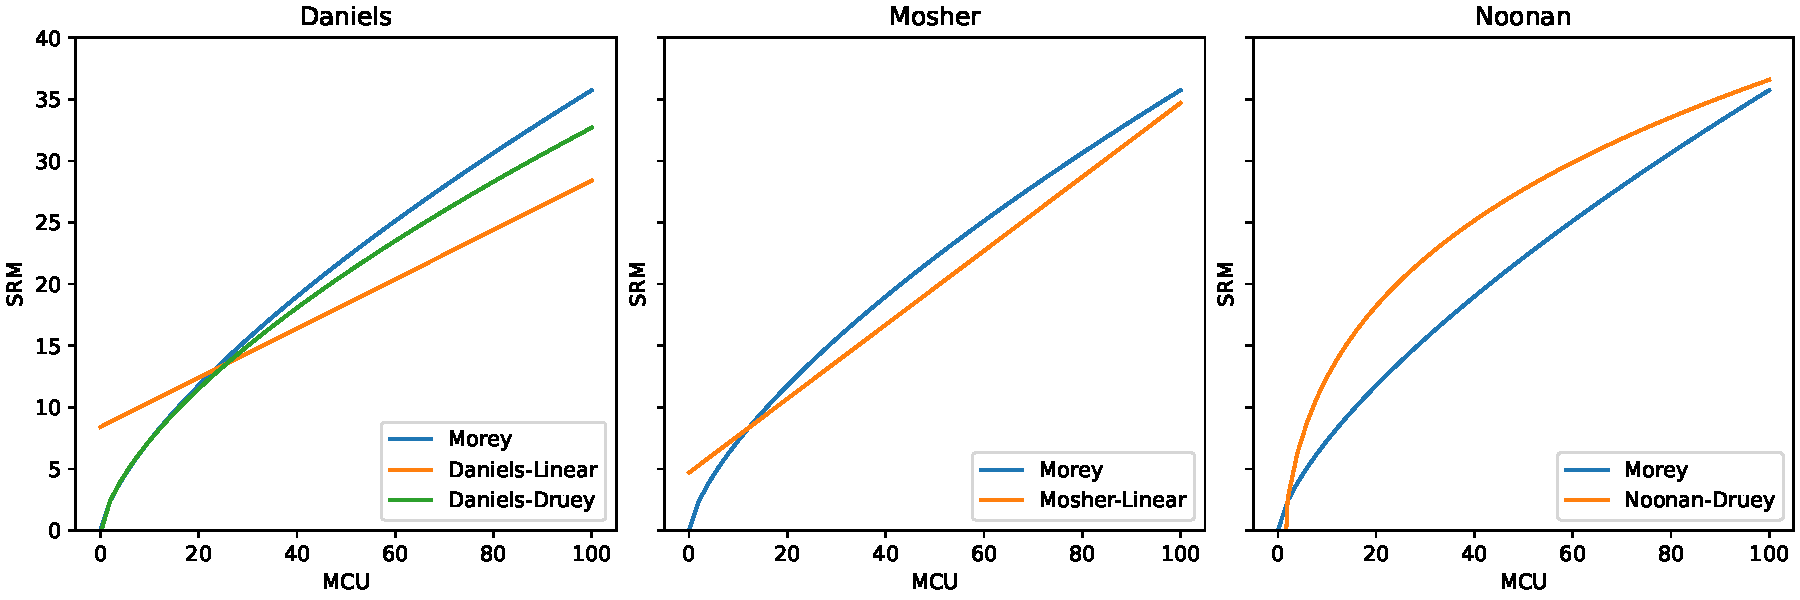
\includegraphics[width=14cm]{graph_srm.pdf}
\caption{Korrelation zwischen SRM und MCU (Ascher, 2022)}
\label{fig:mcucompare}
\end{figure}

\subsection*{Hanghofer (1999)}

\textcite[76]{Hanghofer1999}

Das Modell von Hanghofer basiert auf metrischen Einheiten und bestimmt die MCU nicht in Bezug auf das Volumen der Anstellwürze sondern auf das trockene Schüttungsgewicht (\autoref{eq:mcubasisebc}). Es ist ein Korrekturfaktor für die Stammwürze vorgesehen (\autoref{eq:hanghoferfstw}) sowie ein Korrekturwert für eine übermäßige Zufärbung bei hellen Bieren (\autoref{eq:hanghoferhell}), die laut \textcite{Krueger2019} empierisch ermittelt werden muss und üblicherweise zwischen 2 und 4~EBC liegt. Die Berechnung nach \textcite[78]{Hanghofer2019} erfolgt gemäß \autoref{eq:ebchanghofer}.

\begin{equation}
\MCUEBC = \frac{\sum \text{Malzgewicht}_i \ukg \cdot \text{Malzwürzefarbe}_i \uebc}{\sum \text{Malzgewicht}_i \ukg} 
\label{eq:mcubasisebc}
\end{equation}

\begin{equation}
\fstw = \frac{\text{Stammwürze} \uplato}{9}
\label{eq:hanghoferfstw}
\end{equation}

\begin{equation}
\khell \uebc := \left[2, 4 \right]
\label{eq:hanghoferhell}
\end{equation}

\begin{equation}
\EBC = \MCUEBC \cdot \fstw + \khell
\label{eq:ebchanghofer}
\end{equation}

\subsection*{Krüger (2019)}

Abgesehen vom Korrekturfaktor für die Stammwürze (\autoref{eq:krugerstw}) entspricht das Krüger Modell von den Berechnungsvorschriften weitgehend dem Hanghofer Modell. Es ist jedoch eine weitere Korrektur für die Zufärbung (\autoref{eq:krugerkkd}) über die Kochdauer vorgesehen. Die Berechnung nach \textcite{Krueger2019} erfolgt gemäß \autoref{eq:ebckruger}.

\begin{equation}
\fstw = \frac{\text{Stammwürze} \uplato}{10}
\label{eq:krugerstw}
\end{equation}

\begin{equation}
\kkd \uebc = \text{Kochdauer} \uhour \cdot 1,5 \uebch
\label{eq:krugerkkd}
\end{equation}

\begin{equation}
\EBC = \MCUEBC \cdot \fstw + \khell + \kkd
\label{eq:ebckruger}
\end{equation}

\subsection*{Weyermann (2021)}

Von der Weyermann Mälzerei wird die dem Krüger Modell ähnliche \autoref{eq:ebcweyermann} für Farbvorhersagen eingesetzt. Diese enthält zwei Korrekturen für die Stammwürze in der Form von \autoref{eq:weyermannstw} und \autoref{eq:weyermannkstw}. \parencite{KrausWeyermann2021b}

\begin{equation}
\fstw = \frac{\text{Stammwürze} \uplato}{10}
\label{eq:weyermannstw}
\end{equation}

\begin{equation}
\kstw \uebc = \begin{cases}
0  & \text{für} \quad \text{Stammwürze} \le 7 \uplato, \\
3  & \text{für} \quad 7 \uplato > \text{Stammwürze} \le 10 \uplato, \\
5  & \text{für} \quad 10 \uplato > \text{Stammwürze} \le 15 \uplato, \\
7  & \text{für} \quad 15 \uplato > \text{Stammwürze} \le 20 \uplato, \\
10 & \text{für} \quad 20 \uplato > \text{Stammwürze}. \\
\end{cases}
\label{eq:weyermannkstw}
\end{equation}

\begin{equation}
\EBC = \MCUEBC \cdot \fstw + \kstw
\label{eq:ebcweyermann}
\end{equation}

\subsection*{Modellvergleich}


\parencite{KrausWeyermann2021b}
20 Biere in Weyermann Braumanufaktur. Gemessen und Labo-Messung mit Formel verglichen.
wobei 1 Bier (Export hell) als ausreißwer entfernt wurde.
keine 100 prozen überinstimmung mit labormessung.
Weyermann und Krüger beste Ergebnis.

\begin{table}[H]
\centering
\begin{tabular}{lr}
\toprule
\multicolumn{1}{c}{\textbf{Modell}} & \multicolumn{1}{c}{\textbf{Mittlere Abw. [\%]}} \\
\midrule
Daniels-Linear & -14,4 \\
Krüger & 6,9 \\
Morey & -51,8 \\
Mosher-Linear & -57,2 \\
Weyermann & -2,1 \\
\bottomrule
\end{tabular}
\caption{TODO \parencite{KrausWeyermann2021b}}
\label{table:modelcompareall}
\end{table}

Ausschlagvolumen: 275 Liter


\begin{table}[H]
\centering
\begin{tabular}{lrr}
\toprule
\multicolumn{1}{c}{\textbf{Malz}} & \multicolumn{1}{c}{\textbf{Gewicht [kg]}} & \multicolumn{1}{c}{\textbf{Farbe [EBC]}} \\
\midrule
Pilsner Tennenmalz & 42,8 & 3,75 \\
Carapils & 2,3 & 4,5 \\
Sauermalz & 0,9 & 6 \\
Carabohemian & 0,5 & 195 \\
\bottomrule
\end{tabular}
\caption{Pilsner mit 11,7~°P Stw. \parencite{KrausWeyermann2021c}}
\label{table:pilsner}
\end{table}

\begin{table}[H]
\centering
\begin{tabular}{lrr}
\toprule
\multicolumn{1}{c}{\textbf{Malz}} & \multicolumn{1}{c}{\textbf{Gewicht [kg]}} & \multicolumn{1}{c}{\textbf{Farbe [EBC]}} \\
\midrule
Pilsner Tennenmalz & 38,9 & 3,75 \\
Carapils & 2,4 & 4,5 \\
Sauermalz & 0,9 & 6 \\
Carabohemian & 2,4 & 195 \\
Carafa Typ III & 1,9 & 1400 \\
\bottomrule
\end{tabular}
\caption{Dunkles mit 12,3~°P Stw. \parencite{KrausWeyermann2021c}}
\label{table:dunkles}
\end{table}

\begin{table}[H]
\centering
\begin{tabular}{lrr}
\toprule
\multicolumn{1}{c}{\textbf{Modell}} & \multicolumn{1}{c}{\textbf{Pilsner [EBC]}} & \multicolumn{1}{c}{\textbf{Dunkles [EBC]}} \\
\midrule
Messwert nach EBC & 10 & 82 \\
Daniels-Druey & 7 & 34 \\
Daniels-Linear & 18 & 31 \\
Hanghofer & 10 & 99 \\
Krüger & 11 & 91 \\
Morey & 6 & 36 \\
Mosher-Linear & 11 & 32 \\
Noonan-Druey & 10 & 48 \\
Weyermann & 12 & 92 \\
\bottomrule
\end{tabular}
\caption{TODO \textcite{KrausWeyermann2021c}}
\label{table:modelcompare}
\end{table}

\begin{figure}[h]
\centering
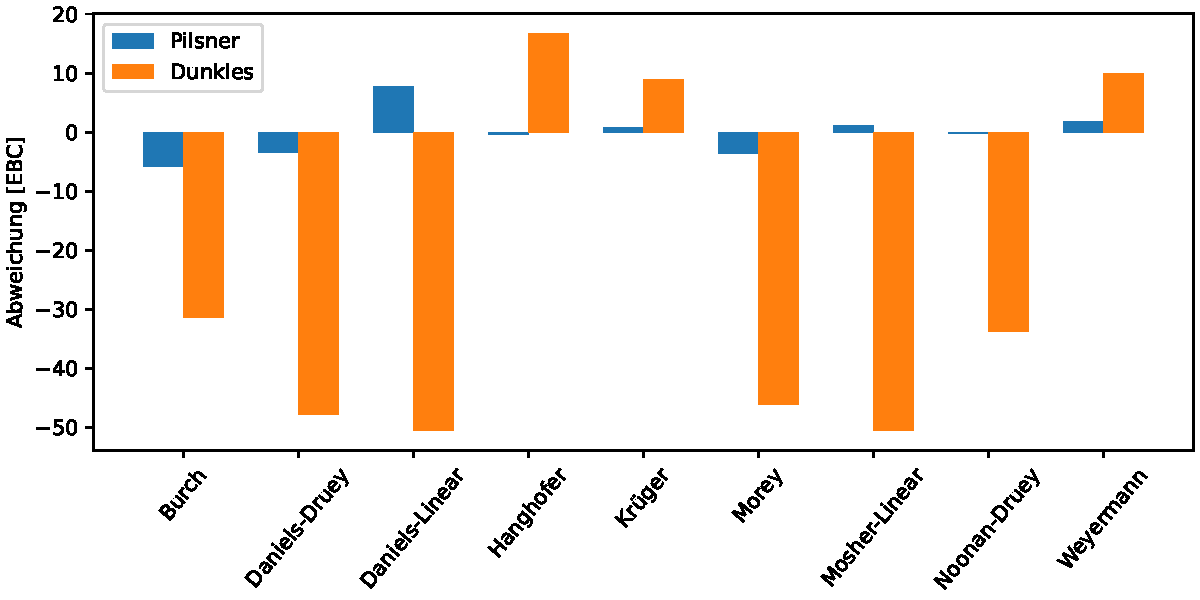
\includegraphics[width=14cm]{graph_dev.pdf}
\caption{TODO (Ascher, 2022)}
\label{fig:modelcompare}
\end{figure}

\section*{Farbsimulation von EBC Werten}

Moussa Clarke

\href{https://github.com/moussaclarke/ebc2hexjs}{Ebc2Hex.js}

\begin{equation}
\SRM = \frac{\max ( 0, \min ( 80, \EBC ) )}{1,97}
\label{eq:srmtor}
\end{equation}

\begin{equation}
R = \min ( 255, \lfloor 280 - \SRM \cdot 5,65 \rceil )
\label{eq:srmtor}
\end{equation}

\begin{equation}
G = \lfloor 0,188349 \cdot \SRM^2 - 13,2676 \cdot \SRM + 239,51 \rceil \\
\label{eq:srmtog}
\end{equation}

\begin{equation}
\begin{split}
B = \max ( 0, \lfloor 0,000933566 \cdot \SRM^4 - 0,0894788 \cdot \SRM^3 + \\ 
3,00611 \cdot \SRM^2 - 40,8883 \cdot \SRM + 183,409 \rceil )
\end{split}
\label{eq:srmtob}
\end{equation}


\section*{Berechnungsbeispiel}

Für einen Sud mit einer Schhüttung bestehend aus 4~kg Pale Ale Malz (5,5~EBC) und 0,25~kg Kara­mell­mal­z (110~EBC) mit einer Stammwürze von 12~°P ist die zu erwartende Bierfarbe abzuschätzen. Berechne diese mithilfe des Weyermann Modells. Unter der Anwendung von \autoref{eq:ebcweyermann} ergibt sich folgender Berechnungsweg:

\begin{align*}
\MCUEBC &= \frac{4 \cdot 5,5 + 0,25 \cdot 110}{4 + 0,25} = 11,6 \\
\fstw &= \frac{12}{10} = 1,2 \\
\kstw &= 5 \\
\EBC &= 11,6 \cdot 1,2 + 5 = 19
\end{align*}

\section*{Zusammenfassung}



\parencite{Bies2010}
\parencite{Tucker2017}
\parencite{Lange2016}

Die relevanten Eckpunkte dieses Artikels sind:

\begin{itemize}
\item Die Farbe eines Bieres und die Würzefarbe eines Malzes werden in EBC auf Basis der Lichtabsorption in einem Spektrophotometers gemessen. Es existieren noch weitere Messverfahren.
\item Viele Faktoren während dem Brau- und Gärvorgang haben neben den eingesetzten Malzen einen signifikanten Einfluss auf die Bierfahre.
\item Es existieren mehrere Berechnungsmodelle, die auf Basis der Schüttung einen EBC Wert bedingt vorhersagen können. Laut einer Versuchsreihe der Weyermann Mälzerei liefern derzeit die Modelle von Weyermann und Krüger die besten Schätzungen.
\item TODO
\end{itemize}

\printbibliography[title=Quellen]

\end{document}
